\chapter{Description de la passerelle}

Comme expliqué dans la section précédente le capteur transmet les informations à la passerelle en utilisant le protocole LoRa. L’objectif principal de la passerelle est la récupération des données transmises par les capteurs, de leur traitement pour finalement procéder au stockage des informations dans une base de données.

La passerelle est composée de deux parties, d’une part le récepteur LoRa également appelé un concentrateur, et d’autre part un ordinateur chargé du traitement des paquets reçus. Le concentrateur LoRa est branché sur un bus SPI relié à l’ordinateur de traitement, lorsqu’un paquet est reçu l’ordinateur hôte récupère ce paquet et effectue le traitement approprié. 

Le logiciel qui fait le traitement des paquets est un « packet forwarder », son travail consiste à récupérer les paquets reçus par le concentrateur LoRa au travers du bus SPI puis de les transférer à un serveur par le biais d’un paquet de type UDP. Le paquet UDP contient des métadonnées diverses, comme le temps de réception du paquet ou encore l’adresse de la passerelle qui l’a reçu ainsi que les données brutes du paquet. Une implémentation de « packet forwarder » open source développée par Semtech est disponible sur internet gratuitement, une multitude d’autres version ont également été créées sur cette base couvrant différent type de cas d’utilisations.

Dans le cadre du travail de Bachelor il s’agira de déterminer quel est le forwarder adapté au matériel et de l’installer sur la passerelle. Un logiciel sera développé dans le cadre du projet, le serveur de paquet, qui réceptionnera les paquets UDP reçu par le packet fordwarder, son travail sera l’extraction des données des paquets reçu depuis le capteur pour enregistrer le tout dans une base de données. Un protocole de communication simple sera défini qui régira le format dans lequel seront transmis les données des capteurs et, si le besoin se manifeste, la gestion d’éventuelles acquittement de transmission des données. Ce protocole sera également géré par le serveur de paquet.

Pour des raisons de simplification le forwarder, le logiciel de traitement des paquets et la base de données seront tous hébergé sur la même machine hôte, c’est-à-dire l’ordinateur de traitement connecté au concentrateur.

La figure~\ref{fig:archi_passerelle} montre l'architecture de la passerelle ainsi que du capteur.

\begin{figure}[htb]
\centering 
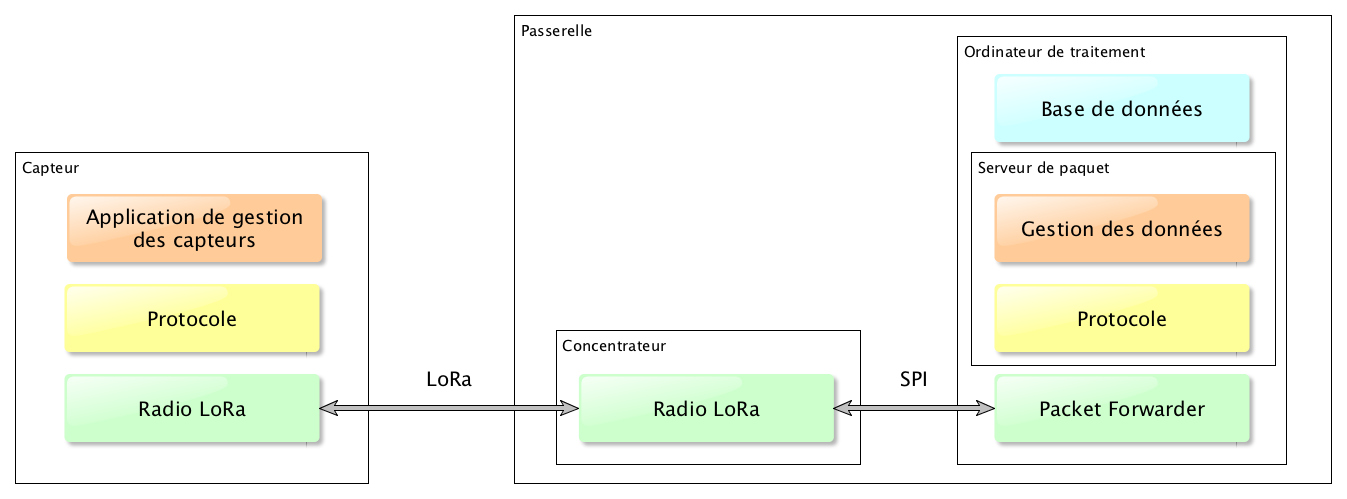
\includegraphics[width=1\columnwidth]{../images/capteur_lora.png} 
\caption[Architecture passerelle]{Architecture logiciel de la passerelle}
\label{fig:archi_passerelle}
\end{figure}

\section{Types de passerelle}

Les passerelles sont divisées en deux groupes, multi canaux (multi channel) et simple canaux (single channel). Les simples canaux sont des passerelles qui se basent sur les mêmes composants LoRa radio que les modules LoRa utilisé pour les nœuds. Puisque ces composants sont destinés aux end-devices ils ne sont capables de gérer qu’un seul canal en réception à la fois, cela vient du fait que la réception qui est prévu uniquement pour les paquets d’acquittements provenant des passerelles, sont toujours envoyé sur le même canal que le paquet envoyé par le nœud, il n’y a donc pas besoin de pouvoir faire de la réception sur plus d’un canal.

L’utilisation d’une passerelle simple canal implique la sélection d’une seule bande de fréquence sur laquelle les paquets de données seront transmis, il faudra veiller à configurer le concentrateur de la passerelle pour qu’il écoute sur cette même fréquence.

Dans le cadre du travail de Bachelor, et dans la mesure où un seul capteur sera développé, une passerelle simple canal sera probablement suffisante pour pouvoir tester le système dans de bonne conditions, il est bien sûre également possible d’utiliser une passerelle multi canaux si le besoin se fait sentir.

\section{Matériel}

Ce chapitre décrit une série de composants qui pourront être utilisé dans l’assemblage final de la passerelle. La sélection des composants exacts utilisés pour le travail de Bachelor se fera au début de la phase de réalisation.

\subsection{Raspberry Pi}

L’élément de base pour la passerelle est un ordinateur de traitement de type Raspberry Pi, mondialement connu, c’est un petit ordinateur à bas coût et proposant des performances très intéressantes. Il a été conçu par la Raspberry Pi Foundation originaire d’Angleterre. Cet ordinateur qui est proposé en différents modèle est utilisé pour tout un tas de projet à travers le monde et du fait de sa petite taille et de ses performances est tout à fait adapté à mon travail de Bachelor. De plus il propose une connexion Ethernet et également WiFi intégrée ainsi que suffisamment de mémoire et d’un processeur capable d’exécuter un système d’exploitation à base de Linux.

Dans le cadre du projet, il faudra installer une distribution Linux sur le Raspberry Pi pour y faire tourner les éléments suivants :

\begin{itemize}
\item Le packet forwarder qui sera en charge de la récupération des paquets LoRa et de leur envoie vers le processus server sous forme de paquet UDP
\item Le server de paquets LoRa qui traitera les données reçues du packet forwarder afin d’extraire les informations relatives au coureur (Position, rythme cardiaque et cadence) pour ensuite les écrire dans une base de données. Le serveur de paquet sera également responsable de la gestion, s’il y en a, du protocole de communication spécialement développé pour ce projet.
\item Le serveur de base de données
\end{itemize}

\begin{figure}[htb]
\centering 
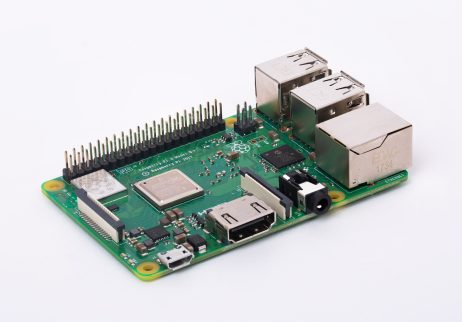
\includegraphics[width=0.8\columnwidth]{../images/RaspberryPi.jpg} 
\caption[Raspberry Pi]{Raspberry Pi - © Raspberry Pi Foundation}
\label{fig:rpi}
\end{figure}

Les caractéristiques du Raspberry Pi sont résumées dans la table~\ref{tab:raspberry_cara}.

\begin{table}[htb]
\caption[Raspberry Pi Caractéristiques]{Caractéristiques du Raspberry Pi 3 Model B+}
\label{tab:raspberry_cara}
\centering
\begin{tabular}{ l | l }
\toprule
Dimensions & 85mm x 49mm \\
\midrule
Microcontrôleur & Broadcom BCM2837B0 – Cortex-A53 64-bit \\
\midrule
Oscillateur & 1.4 Ghz \\
\midrule
Stockage & Carte SD \\
\midrule
RAM & 1 GB SDRAM \\
\midrule
WiFi & 802.11 b/g/n/ac \\
\midrule
Prix & 34.50 CHF\\
\bottomrule 
\end{tabular}
\end{table}

\subsection{Dragino LoRa Hat}

Cette configuration est idéale pour une passerelle de type simple canal facile à mettre en place. 
Au Raspberry Pi viendra se coupler un module qui va gérer la communication LoRa, ces modules d’extension se nomment souvent des hats, ils sont conçus pour pouvoir se ficher au-dessus du Raspberry Pi comme un chapeau. Il en existe plein de type différent proposant tout un panel de fonctionnalité. 

Le module d’extension en l’occurrence le Dragino LoRa Hat contient un module HopeRF RFM95W qui propose une interface SPI à un module radio LoRa SX1276, un composant similaire proposé sur la pluparts des solutions décrites dans la section~\ref{desc_capteur} des capteurs. De plus ce module d’extension est également équipé d’un module GPS dont l’exploitation pourrait être intéressante dans une optique produit, afin de pouvoir localiser également les passerelles, cependant dans le cadre du travail de Bachelor cet aspect ne sera pas traité.

\begin{figure}[htb]
\centering 
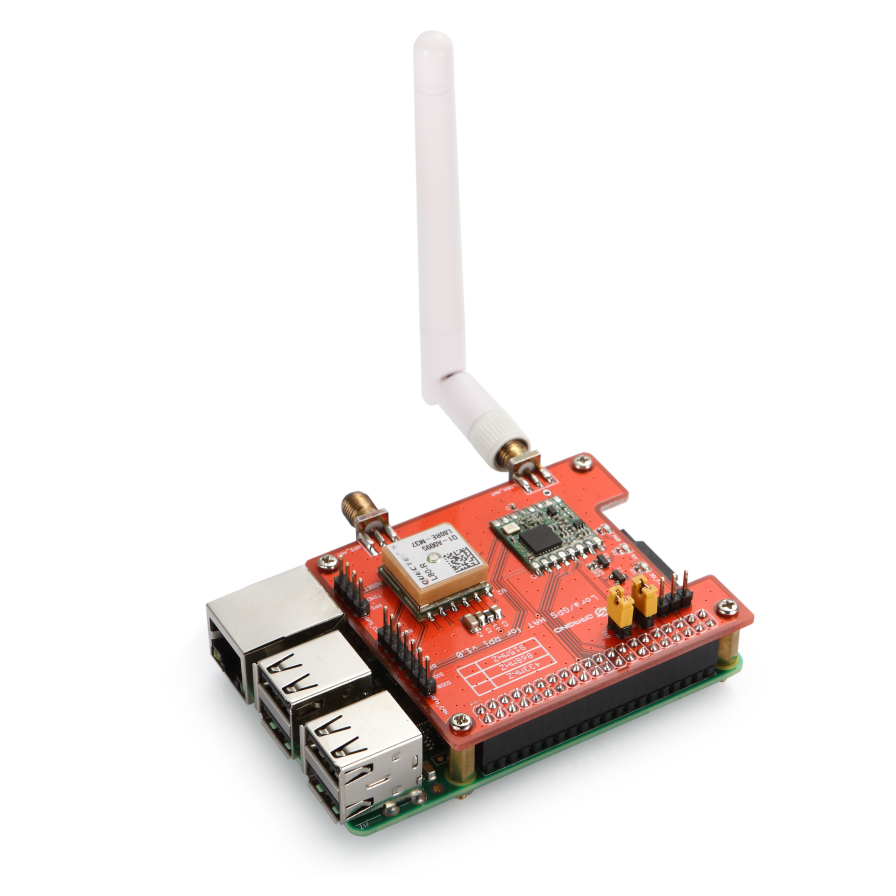
\includegraphics[width=0.5\columnwidth]{../images/RaspberryPI_DraginoHat.png} 
\caption[Raspberry Pi]{Raspberry Pi et son Dragino LoRa hat - © Dragino}
\label{fig:rpi_dragino_hat}
\end{figure}

Les caractéristiques du Dragino Hat sont résumées dans la table~\ref{tab:dragino_cara}.

\begin{table}[htb]
\caption[Dragino Hat Caractéristiques]{Caractéristiques du Dragino LoRa Hat}
\label{tab:dragino_cara}
\centering
\begin{tabular}{ l | l }
\toprule
Dimensions & 60mm x 53mm x 25mm \\
\midrule
LoRa & SX1276 \\
\midrule
Type de passerelle & Simple canal \\
\midrule
Prix & 38.90 CHF \\
\bottomrule
\end{tabular}
\end{table}

L’avantage de la solution Dragino LoRa Hat est principalement son coût peu élevé. Le désavantage étant qu’il ne peut être utilisé uniquement en mode simple canal et donc limite le nombre de canal qu’il est possible d’utiliser en parallèle.

\subsection {IMST iC880A}

L’iC880A est un concentrateur capable de fonctionner en mode multi canaux. Il peut recevoir des paquets utilisant des facteurs d’étalement différents sur 8 canaux différents au maximum, le tout en parallèle. Un de ses avantages principaux est qu’il est capable de gérer différents étalements et largeur de bandes ce qui rend possible l’utilisation de l’adaptative data rate (ADR) proposé par le protocole LoRaWAN et qui permet au serveur réseau d’adapter le taux de transferts des nœuds de manière dynamique et ainsi rendre le réseau plus performant. Dans la mesure ou le projet ne va utiliser que la couche radio LoRa, cet argument n’entre donc pas en ligne de compte.

De manière similaire au Dragino LoRa Hat, ce concentrateur travail conjointement avec un ordinateur de traitement, le Raspberry Pi par exemple qui traitera les paquets LoRa qui sont reçus.

\begin{figure}[htb]
\centering 
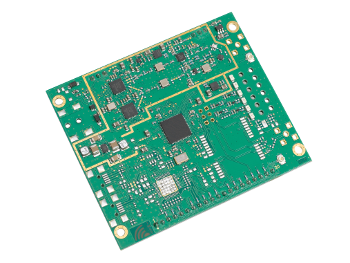
\includegraphics[width=0.5\columnwidth]{../images/iC880A.png} 
\caption[IMST iC880A]{IMST iC880A -© IMST}
\label{fig:imst_ic880a}
\end{figure}

Les caractéristiques du Dragino Hat sont résumées dans la table~\ref{tab:dragino_cara}.

\begin{table}[htb]
\caption[IMST iC880A Caractéristiques]{Caractéristiques du IMST iC880A}
\label{tab:imst_cara}
\centering
\begin{tabular}{ l | l }
\toprule
Dimensions & 79.8mm x 67.3mm \\
\midrule
LoRa & SX1301 \\
\midrule
Type de passerelle & Multi canaux \\
\midrule
Prix & 142 CHF \\
\bottomrule
\end{tabular}
\end{table}

Le principal avantage de cette passerelle est le fait qu’elle propose une solution multi canal, avec la gestion de 8 canaux en parallèle il devient donc possible de gérer plusieurs communications avec différents nœuds à la fois.
